{
{\sffamily
For at beskrive integrationen og samspillet mellem en kørsel og
databasen vil der følge en beskrivelse af de vigtige kald mellem 
start.py og databasen. 
}
Start.py er distributør af arbejde til de andre dele af programkoden.
Diagram \ref{start_workflow} og pseudokode \ref{pseudo_workflow} giver et overblik over hvad der bliver
forklaret i resten af dette kapitel. 
\begin{figure}[h!]
	\begin{center}
		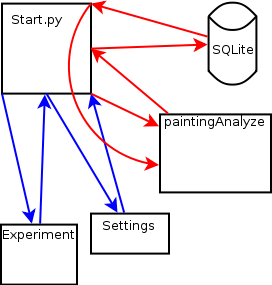
\includegraphics[scale=0.5]{afsnit/implementation/billeder/workflow_start_py.png}
	\end{center}
	\caption{De blå pile er ting, som sker en enkelt gang, mens de blå
	\label{start_workflow}
	bliver gentaget indtil der ikke er flere billeder at arbejde på}
\end{figure}
\begin{lstlisting}[caption={Pseudokode for
start},frame=tb,label={pseudo_workflow}]
cuts = experiment.generateCuts()
experiment.setSettings(settings)
experiment.setGlobalSettings(globalSettings)
db = Database(globalSettings)
db.construct(Database)
run = m.createNewRun(settings)
paintings = m.Painting.select(m.Painting.q.form=="painting")
for painting in paintings:
	paintingContainer = Painting(painting)
	paintingContainer.setResults(paintingAnalyzer.analyze(paintingContainer,settings))
	m.saveResults(run.id,paintingContainer)
\end{lstlisting}
\subsection{Eksperimenter}
Eksperimenterne er til for at samle konfigurationen af en kørsel.
Kravene til et eksperiment er at den skal have mindst tre metoder:
generation af snit, sætte globale indstillinger samt sætte
kørselsspecifikke indstillinger. \ref{pseudo_experiment} er et eksempel
på hvordan et eksperiment evt. kunne se ud.
\begin{lstlisting}[caption={Pseudokode for et
experiment, som checker på $\varPhi$},frame=tb,label={pseudo_experiment}]
def generateCuts():
	cuts = [goldenLibrary.PHI,2/3]
	return cuts
def setSettings(settings):
	settings.setMarginPercentage(0.024)
	return 0
def setGlobalSettings(globalSettings):
	return 0
\end{lstlisting}
%Settings 
\subsection{Globale indstillinger}
Globale indstillinger er informationer, som har brug for at blive gemt
mellem kørsler. I det nuværende tilfælde er det placeringen på databasen og
csvfilen fra wga.hu, det kunne udvides til også at inkludere placeringen
af billederne istedet for at være fastdefineret.

\subsection{Kørselsindstillinger}
Disse indstilinger kan afvige i forskellige kørsler, det er variable
hvis indstillinger betyder meget for resultaterne og derfor er vigtige
at kunne ændre. De består af tærskelværdier for floodfill og
kantdetektion samt størrelsen på margin\ref{terskelverdi}, de snit, som
skal undersøges og hvilken metode, der skal benyttes.

\subsection{Konstruktion af databasen}
Databasen bliver selvfølgelig ikke rekonstrueret ved enhver kørsel, men
undtagen i speciel tilfældet at der skal skabes en
testdatabase; se \ref{test_db}, vil den kommaseparede fil blive gennemløbet.
Det er værd at bemærke at dette også betyder at databasen ikke kan
håndtere at blive afbrudt i dette stadie første gang den bliver kørt.
Omvendt giver det mulighed for at den kommeseparerede fil kan opdateres uden nogen
problemer. Og da billederne automatisk bliver hentet hvis de mangler
giver det også mulighed for at flytte databasen over til en anden
maskine uden nogen problemer. Følgende pseudokode forklare hvordan
konstruktionen af databasen foregår.
\begin{lstlisting}[caption={Pseudokode for database
initialisering},frame=tb,label={pseudo_init_db}]
csvfile = open(Settings.csvfilelocation)
for line in csvfile:
	line = parser.parse(line)
	if not os.path.isfile(line.path):
		download(line.url)
	if database.Painting.select(database.Painting.url==line.url).count() == 0:
		painting = database.Painting(line)
\end{lstlisting}
\subsubsection{Parsing af kommasepareret fil}
I filen gives endvidere mange oplysninger, om den enkelte artikel samt
dennes kunstner.  Vi har konstrueret en parser, som trækker disse
informationer ud fra filen og lægger dem ind i databasen. Da vi primært
vil beskæftige os med malerier, vil vi nu blot omtale kunstartikler som
malerier.

Den konstruerede parser, til den kommaseparerede fil, er dog ret grov,
da folkene bag \cite{wgahu} ikke har lagt meget vægt på, at være
konsistente i deres formulering af en kunstners fødsels- og dødsår eller
en genstands dimensioner. En følge deraf er, at nogle kunstnere, hvor
\cite{wgahu} ikke har en klar indikation af dennes levealder, ikke
bliver registreret i databasen. Vi kan dog stadig slå kunstneren op ved
at bruge feltet ``timeline'', som angiver hvilken periode kunstneren
tilhører. Vi har i enkelte tilfælde, set os nødsaget til at rette i den
kommaseparerede fil, hvor der er blevet indsat tegn, som helt umuliggør
korrekt parsing af filen, såsom ekstra komma eller semikolon.

\subsubsection{Databasens opbygning}
Ved at bruge \emph{SQLObject} er det ligetil at konstruere tabeller i
databasen. Vi har i afsnit \ref{section_database} givet det database
skema som vi opbygger databasen efter. I kodeboks
\ref{code_tabel_artist} er vist hvordan tabellen \texttt{artist}
konstrueres ved brug af \emph{SQLObject} i Python.

\begin{lstlisting}[caption={Pythonkode for oprettelse af tabeller i
    databasen.}, captionpos=b, label={code_tabel_artist}, frame=tb,
    breaklines=false, float=hb]
import sqlobject as s

class Artist(s.SQLObject):
    "
    _id_, name, born, died, school, timeline
    "
    name = s.StringCol()
    born = s.IntCol()
    died = s.IntCol()
    school = s.StringCol()
    timeline = s.StringCol()
\end{lstlisting}

Når man vil oprette en ny kunstner i databasen gøres det som vist
i kodeboks \ref{code_new_artist}.

\begin{lstlisting}[caption={Oprettelse af en kunstner i databasen.},
    captionpos=b, label={code_new_artist}, frame=tb, breaklines=false,
    float=h]
# Init variables
name = "Homer Simpson"
born = 1968
died = 2000
school = "Springfield"
timeline = "1950-2000"

# Create the artist in the database
Artist(name=name, born=born, died=died, school=school, timeline=timeline)
\end{lstlisting}

\emph{SQLObject} opretter automatisk et id-felt til alle tabeller i
databasen. Vi kan udnytte dette til at lave \emph{foreign keys} i
tabellerne. Vi viser i kodeboks \ref{code_tabel_result} hvordan tabellen
\texttt{result} oprettes i databasen, hvor det er interessant at bemærke
hvorledes de to \emph{foreign keys} oprettes.

\begin{lstlisting}[caption={Pythonkode for oprettelse af \emph{foreign
    keys} i databasen.}, captionpos=b, label={code_tabel_result}, frame=tb,
    breaklines=false, float=h]
class Result(s.SQLObject):
    "
    _id_, ^runId, ^paintingId, cutRatio, cutNo, numberOfRegions
    "

    run = s.ForeignKey('Run')
    painting = s.ForeignKey('Painting')
    cutRatio = s.FloatCol()
    cutNo = s.IntCol()
    numberOfRegions = s.IntCol()
\end{lstlisting}
\subsubsection{Testdatabase}\label{test_db}
For at alle kan arbejde på det samme billeder undervejs i udviklingen er
det muligt at konstruere en lille database, dette gøres ved at sætte
testdatabase variablen til True. Databasen vil kun vokse til count
variablen. En fuld beskrivelse kan findes i \ref{brugervejl_test_db}


\subsection{Analysen}
Analysen bliver kørt på alle billeder, som har typen "painting" i den
kommaseparerede fil. Som beskrevet i linje 8-10 i \ref{pseudo_workflow}
så bliver billedet sendt igennem Painting klassen, hvor det bliver
konverteret til et \emph{Opencv} billede. Når det er konverteret sendes
det til paintingAnalyser, hvis formål er at sende det videre til
udtrækning af regioner. Efter alle regioner er trukket ud gemmes
resultaterne i databasen.

\subsection{Genskabelse af parametre og resultater}
At kunne genskabe de fundne resultater fra en analyse har meget stor
betydning, dels for at kunne udtage stikprøver i udviklingen af hele
programmet, men også for at kunne fremvise grafiske resultater. Vi har
allerede været inde på, at man for at kunne genskabe et resultat, skal
vide hvilke parametre der oprindeligt har været brugt. Ovenstående
databaseskema gør det let at hente disse parametre ud. Hvis vi får et
resultat med overraskende mange regioner og gerne vil undersøge dette
tilfælde, har vi metoder til rådighed der giver os lige nøjagtig de
informationer vi har brug for at vise dette grafisk. Helt konkret har vi
metoderne vist i listing \ref{rekonst_koersel} til rådighed.

\vspace{0.5cm}
\begin{lstlisting}[caption={Metoder til rekonstruktion af kørsler},captionpos=b,label={rekonst_koersel},numbers=none]
def getSettingsForRunId(runId):
    """Return the settings instance for a given run"""
    pass

def getCutRatiosForRunId(runId):
    """Return the list of cut ratios for a given run"""
    pass

def getSettingsForResultId(resultId):
    """Return the settings instance for a given result"""
    pass

def getSettingsForRegionId(regionId):
    """Return the settings instance for a given region"""
    pass

def getCutRatioForRegionId(regionId):
    """Return the list of cut ratios for a given region"""
    pass

def getCutNoForRegionId(regionId):
    """Return the cut number for a given region"""
    pass

def getRegionsForResultId(resultId):
    """Return the list of regions for a given result"""
    pass
\end{lstlisting}

Selvom metoderne i listing \ref{rekonst_koersel} ikke viser noget
egentlig kode, bør det ud fra sammenhængen være klart hvad disse metoder
gør. Alle metoder der starter med \texttt{getSettings} returnerer
klassen \texttt{Settings} som vist i listing \ref{settings_klassen} med
indstillinger tilpasset den enkelte forespørgelse.
\vspace{0.5cm}
\begin{lstlisting}[caption={Settings-klassen med standardindstillinger},captionpos=b,label={settings_klassen},numbers=none]
class Settings:
    """These are the default settings for the analysis"""
    edgeThreshold1 = 78
    edgeThreshold2 = 2.5 * edgeThreshold1
    lo = 4
    up = 4
    cutRatios = None
    marginPercentage = 0.009
    method = 'naive'
    ...
\end{lstlisting}

Det ses at vi har mulighed for at trække de fundne regioner ved et
snit ud og vi behøver derfor ikke at køre nogen analyse på billedet hvis
vi blot ønsker at få de fundne regioners begrænsende areal vist. I dette
tilfælde kan vi nøjes med at forespørge databasen om de regioner der er
tilknyttet et snit vi gerne vil undersøge og traversere gennem den liste
af regioner vi får tilbage. Hver region er repræsenteret som en klasse
hvor vi kan trække rektanglet ud og vi bruger da \emph{OpenCV} til at
tegne rektanglet på det tilknyttede billede.
}
% vim: set tw=72 spell spelllang=da:
